%%%%%%%%%%%%%%%%%%%%%%%%%%%%%%%%%%%%%%%%%
% University/School Laboratory Report
% LaTeX Template
% Version 3.0 (4/2/13)
%
% This template has been downloaded from:
% http://www.LaTeXTemplates.com
%
% Original author:
% Linux and Unix Users Group at Virginia Tech Wiki 
% (https://vtluug.org/wiki/Example_LaTeX_chem_lab_report)
%
% License:
% CC BY-NC-SA 3.0 (http://creativecommons.org/licenses/by-nc-sa/3.0/)
%
%%%%%%%%%%%%%%%%%%%%%%%%%%%%%%%%%%%%%%%%%

%----------------------------------------------------------------------------------------
%	PACKAGES AND DOCUMENT CONFIGURATIONS
%----------------------------------------------------------------------------------------
\documentclass{article}
\usepackage{amsmath}
\usepackage{amsfonts}
\usepackage{amssymb}
\usepackage{siunitx} % Provides the \SI{}{} command for typesetting SI units
\usepackage{graphicx} % Required for the inclusion of images
\setlength\parindent{0pt} % Removes all indentation from paragraphs
\def\thesection{\Alph{section}} % make the secions be index by letters
\usepackage[section]{placeins} % make sure figures are placed in the correct section
\usepackage{pdfpages}
\usepackage[version=3]{mhchem} % chemistry typesetting
\usepackage{pdfpages} %include PDF pages
%\usepackage{times} % Uncomment to use the Times New Roman font

%----------------------------------------------------------------------------------------
%	DOCUMENT INFORMATION
%----------------------------------------------------------------------------------------
\title{Safety Plan \\ Pyralis Engine \\ MIT Rocket Team} % Title
\author{Matt Vernacchia, President\\James Logan, Vice President\\Connie Liu, Treasurer\\Ben Corbin, Safety Officer
\\\\ Prof. Paulo Lozano, Faculty Advisor} % Author name
\date{ \today } % Date for the report

%----------------------------------------------------------------------------------------
% THE BODY OF THE REPORT
%---------------------------------------------------------------------------------------

\begin{document}
\maketitle
This document presents an analysis of the risks facing MIT Rocket Team members during the manufacturing and testing of the Pyralis rocket engine, and strategies for mitigating those risks.
\section{Machining Hazards}
Only team members who have been trained by the MIT AeroAstro Gelb Lab staff will be allowed to use machine or power tools. Members will be encouraged to receive additional training from the MIT Hobby Shop or Edgerton Center.

\section{Pressurized Apparatus Hazards}
\subsection{Commercial Pressure Vessels}
We will use equipment and techniques approved by our gas supplier, Airgas, to connect commercial gas supply pressure vessels to our device.
\subsection{Custom Pressure Vessels}
We will custom-manufacture pressure vessels to store fuel and oxidizer in the rocket during launch and flight. To achieve the low mass needed for flight, these vessels must be designed with a yield strength safety margin of $1.5$ to $2.5$. To protect personnel from injury, our launch and test operations will be conducted under the assumption that, once pressurized, the flight tanks may fail at any time. Blast-proof barriers will be kept between people and the flight tanks at all times when the tanks are pressurized.

\section{Engine Test Plan}
\subsection{Facilities}
All test firings of the engine will be conducted within a blast chamber capable of withstanding an explosion equivalent to $\SI{2}{lbs}$ of TNT ($\SI{4.2}{\mega\joule}$).
\subsection{Planning}
A detailed experiment plan and safety check-list will be prepared for each test. These documents will be approved by the blast chamber operator (John Kane) and the club's faculty advisor before the test is conducted.
\subsection{Auditory Hazard}
The firing of the rocket engine may be dangerously loud. All people involved in an engine test will wear hearing protection for the duration of the firing.
\subsection{Equipment Layout}
\begin{figure}[h!]
\centering
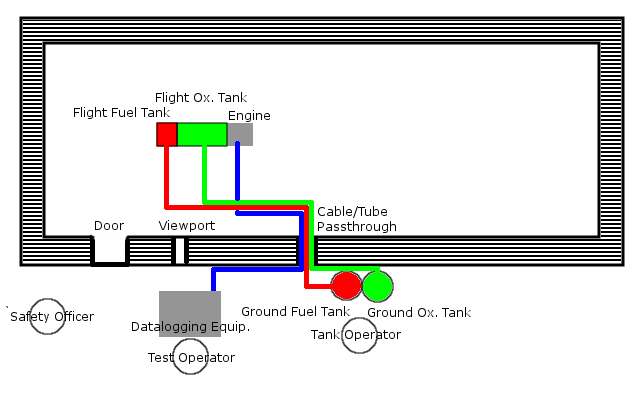
\includegraphics[width = \textwidth]{blast_chamber_layout.png}
\caption{Positions of equipment and people involved in a rocket engine firing} 
\label{layout}
\end{figure}
\subsection{Procedure}
The following sequence of events will occur during a nominal engine test:
\begin{enumerate}
\item The engine and flight tanks will be installed in the chamber.
\item The data-logging system and ground tanks will be set up outside the chamber. The ground tanks will be strapped to a wall or rack so that they do not fall over.
\item Propellant fill lines and data cables will be routed through the pass-through in the chamber wall. They will be connected to the equipment within the chamber.
\item The data cables will be connected to the data-logging equipment and the Test Operator will perform a checkout of all sensors.
\item The Tank Operator will activate the chamber ventilation system and verify that it is functioning.
\item All people will exit the chamber.
\item The Safety Officer will verify that all people have left the chamber and will then close the chamber door.
\item The Tank Operator will connect the propellant feed lines to the ground tanks.
\item With approval from the Safety Officer, the Tank Operator will open a valve to transfer propellant from the ground tanks to the flight tanks. Once the flight tanks are filled, the Tank Operator will shut off the connection between the ground tanks and flight tanks.
\item With approval from the Safety Officer and Tank Operator, the Test Operator will fire the engine.
\item After the firing is complete, the chamber will be allowed to ventilate until:
\subitem A \ce{CO} sensor within the chamber indicates that the \ce{CO} concentration has reached a safe level.
\subitem Temperature sensors on the engine indicate that the exterior surfaces have cooled to $\SI{40}{\celsius}$. 
\item The Safety Officer will the open the chamber door.
\item All equipment will be recovered from within the chamber.
\end{enumerate}
In the event that a test must be aborted while the flight tanks are pressurized the following procedure will be followed:
\begin{enumerate}
\item The Tank Operator will remotely open purge valves on the flight tanks.
\item The Test Operator will examine the tank pressure sensor readings to verify that the tanks have been purged.
\item The chamber will be allowed to ventilate for $\SI{10}{\minute}$.
\item The Safety Officer will open the chamber door.
\end{enumerate}

\section{Propellant Toxicity}
\subsection{Ethane Fuel}
Ethane is not known to have toxic effects, it only presents a health hazard as a simple asphyxiant \cite{EthaneMSDS}.
\subsection{Nitrous Oxide Oxidizer}
Nitrous oxide presents a hazard as a simple asphyxiant and prolonged exposure may cause damage to the reproductive system, upper respiratory tract, and central nervous system \cite{N2OMSDS}. Nitrous oxide also acts as a dissociative anaesthetic when inhaled. Acute effects of overexposure include decreased mental performance, audiovisual ability, and manual dexterity, while long-term exposure can cause vitamin B-12 deficiency \cite{NIOSH}. These risks can be minimized by using adequate ventilation during processes which may leak nitrous oxide. Team members who work with nitrous oxide processes will be provided with vitamin B-12 supplements.

\section{Exhaust Toxicity}
Below is an estimate of the chemical constituents of the exhaust for burning ethane and nitrous oxide in a 4:1 ratio by mass at $\SI{5}{\mega\pascal}$ chamber pressure.
These values were calculated using NASA's CEARUN combustion simulator.\\
\begin{tabular}{ l | c | c | c | c }
Species & Mole Frac in Exhaust & Molar Mass & Present in \SI{1}{\mole} Exhaust & Produced by \SI{1}{\kg} Prop.\\
\hline
CH4 & $0.012$ & \SI{16}{\gram\per\mole} & \SI{0.192}{\gram} & \SI{3.29}{\gram} \\
CO  & $0.158$ & \SI{28}{\gram\per\mole} & \SI{4.424}{\gram} & \SI{75.8}{\gram} \\
CO2 & $0.074$ & \SI{44}{\gram\per\mole} & \SI{3.256}{\gram} & \SI{55.8}{\gram} \\
HCN & $\num{2.3e-7}$& \SI{27}{\gram\per\mole} & \SI{6.21d-6}{\gram} & \SI{1.1d-4}{\gram} \\
H2  & $0.317$ & \SI{2}{\gram\per\mole}  & \SI{0.634}{\gram} & \SI{10.9}{\gram} \\
H2O & $0.056$ & \SI{18}{\gram\per\mole} & \SI{1.008}{\gram} & \SI{17.3}{\gram} \\
N2  & $0.362$ & \SI{28}{\gram\per\mole} & \SI{10.136}{\gram} & \SI{173.8}{\gram} \\
C(gr)&$0.021$ & \SI{12}{\gram\per\mole} & \SI{0.252}{\gram} & \SI{4.32}{\gram} \\
\end{tabular}
\\
Of these by-products, hydrogen cyanide (\ce{HCN}) and carbon monoxide (\ce{CO}) are toxic to humans.\\
\subsection{Hydrogen Cyanide}
According to \cite{HCNtox}:\\
`` Exposure to low concentrations may result in a range of non-specific features including
headache, dizziness, throat discomfort, chest tightness, skin itching and eye irritation and 
hyperventilation. With more substantial exposures, features may include severe 
dizziness (near syncope).\\
Exposure to a massive concentration of hydrogen cyanide gas may render an individual 
unconscious within seconds [10, 11] and may lead to coma and death within minutes."\\
The $LD_{50}$  of \ce{HCN} in rats is \SI{3}{\milli\gram\per\kg} by oral ingestion and 
$\SI{158}{\milli\gram\per\cubic\metre}$ for $\SI{60}{\minute}$ of inhalation exposure \cite{HCNtox}.
The amount of \ce{HCN} the combustion process will produce, $\SI{0.11}{\milli\gram}$ per kilogram of propellant,
is well below these levels. The smoke from one cigarette contains approximately the same amount of \ce{HCN} \cite{HCNtox}.
Therefore it is no expected that \ce{HCN} will be a significant source of exhaust toxicity.\\
\subsection{Carbon Monoxide}
Carbon monoxide (CO) is toxic by inhalation, and damages the heart, lungs, blood, cardiovascular system and nervous system \cite{COtox}.
Combustion of $\SI{1}{\kg}$ is expected to produce $\SI{75.8}{grams}$ of \ce{CO}. 
The OSHA ceiling exposure limit for \ce{CO} is $\SI{200}{\milli\gram\per\cubic\metre}$ \cite{COtox}. 
Combusting several kilograms of propellant within a blast chamber without ventilation would produce concentrations exceeding this level. 
Therefore blast chamber tests of the combustion process must be adequately ventilated to prevent \ce{CO} poisoning.

\begin{thebibliography}{9}
	\bibitem{EthaneMSDS} Ethane Material Safety Data Sheet. \emph{Airgas.} http://www.airgas.com/documents/pdf/001024.pdf.
	\bibitem{N2OMSDS} Nitrous Oxide Material Safety Data Sheet. \emph{Airgas.} http://www.airgas.com/documents/pdf/001042.pdf.
	\bibitem{NIOSH} Criteria for a Recommended Standard: Occupational Exposure to Waste Anesthetic Gases and Vapors. \emph{Centers for Disease Control and Prevention.} http://www.cdc.gov/niosh/docs/1970/77-140.html.
	\bibitem{HCNtox} Hydrogen Cyanide Toxicological Overview. \emph{UK Health Protection Agency.} http://www.hpa.org.uk/webc/HPAwebFile/HPAweb\_C/1202487078453.
	\bibitem{COtox} Carbon Monoxide Material Safety Data Sheet. \emph{Airgas.} http://www.airgas.com/documents/pdf/001014.pdf.
\end{thebibliography}
\end{document}
